\chapter{Methodology}\label{chap:Methodology}

\section{Chapter Overview}\label{sec:method_overview}

This chapter specifies the methodology of an affect-informed adaptive tutoring framework that operates as a two-stage pipeline. The first stage is a perception module that performs \ac{FER} on short webcam clips of the learner. The second stage is an adaptive tutoring system that consumes the \ac{FER} output to select pedagogical actions for the learner in real time.

The \ac{FER} module maps each input clip to a four-dimensional affect vector whose components correspond to Boredom, Engagement, Confusion, and Frustration. These four states are the academic affective states annotated in the dataset used in this thesis. Each component of the vector is a continuous score in the interval $[0,1]$ produced by an independent sigmoid output, so the four scores may be simultaneously high and support co-occurring affective states.

The output of the \ac{FER} module is passed directly into the downstream adaptive decision-making system. That system is formulated as a \ac{MDP} and is solved with a \ac{DQN} agent. The four-dimensional affect vector produced by the \ac{FER} module forms part of the state representation observed by the \ac{DQN} agent at each decision step, alongside the learner's knowledge and engagement signals. The formal definition of the \ac{MDP}, the action space, the reward function, and the training procedure of the \ac{DQN} agent are presented in the adaptive tutoring methodology that follows in Section~\ref{sec:method_rl_chapter}; the present chapter is concerned with the perception stage and with the data-flow interface that connects it to the decision stage.

\begin{figure}[H]
    \centering
    \makebox[\textwidth][c]{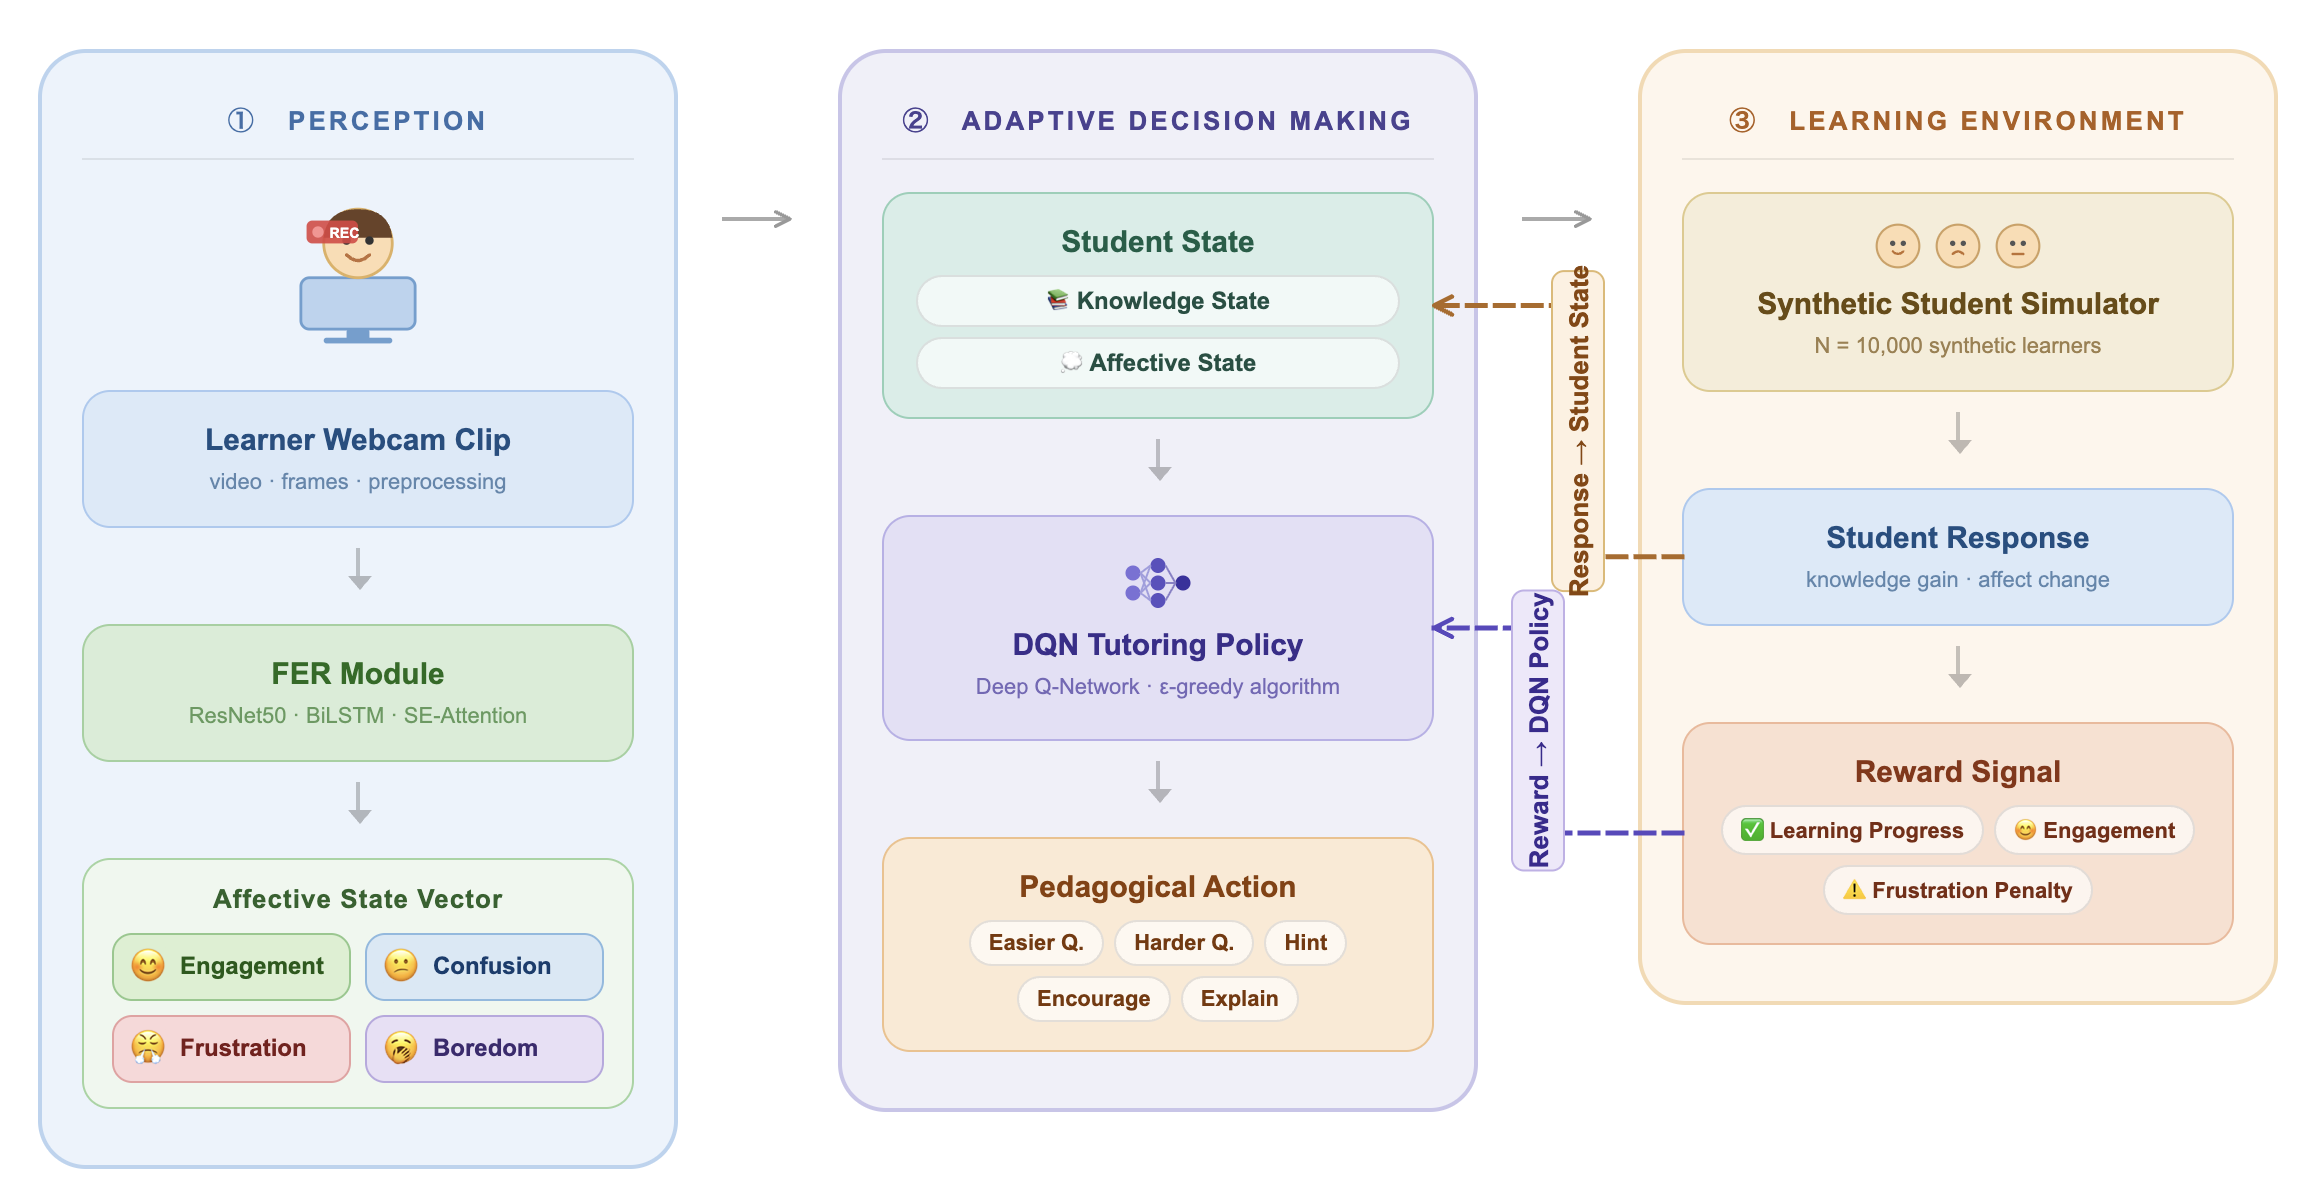
\includegraphics[width=1.25\textwidth,keepaspectratio]{Figures/system_overview.png}}
    \caption{Affect-informed adaptive tutoring framework. The Perception zone maps a learner webcam clip to an affective state vector over Boredom, Engagement, Confusion, and Frustration. The Adaptive Decision Making zone combines this vector with the learner's knowledge state to form the student state consumed by the \ac{DQN} tutoring policy, which selects a pedagogical action. The Learning Environment zone houses the synthetic student simulator and the reward signal that closes the reinforcement-learning loop.}
    \label{fig:system_overview}
\end{figure}

The rest of this chapter is organised as follows. Section~\ref{sec:method_dataset} describes the dataset and label structure. Section~\ref{sec:method_preparation} describes the data preparation pipeline applied before training, including the ordinal-to-binary label mapping. Section~\ref{sec:method_architecture} presents the \ac{FER} architecture component by component and summarises the design elements of the proposed model. Section~\ref{sec:method_training} describes the training and evaluation protocol applied to the \ac{FER} module, including the loss function, the imbalance-handling strategy, the optimisation procedure, the per-label threshold tuning, and the evaluation metrics. Section~\ref{sec:method_rl_chapter} then specifies the adaptive tutoring methodology that consumes the \ac{FER} output, including the Markov Decision Process formulation, the \ac{DQN} agent, and the synthetic student simulator used for training and evaluation.

\section{Dataset Description}\label{sec:method_dataset}

The \ac{FER} module is trained and evaluated on the \ac{DAiSEE} dataset~\cite{gupta_daisee_2016}. \ac{DAiSEE} is a publicly available collection of approximately $9{,}068$ short webcam clips of learners recorded in study-like conditions. Each clip is annotated for four academic affective states: Boredom, Engagement, Confusion, and Frustration~\cite{gupta_daisee_2016}.

The annotation scheme assigns each of the four states an ordinal intensity level on the integer scale $\{0,1,2,3\}$, corresponding respectively to absent, slight, moderate, and very strong manifestations of the state. In this thesis these ordinal annotations are mapped to binary present/absent labels following the adaptation policy of Malekshahi et al.~\cite{malekshahi_engagement_2024}; the conversion rule is formalised in Section~\ref{sec:method_preparation}.

The task is formulated as a multi-label binary classification problem. A single clip can be marked positive for several states at the same time, so the four binary labels are predicted independently and may co-occur on the same clip~\cite{gupta_daisee_2016}.

The dataset is partitioned into the official \ac{DAiSEE} training, validation, and test splits as released by Gupta et al.~\cite{gupta_daisee_2016}. The training set contains $5{,}358$ clips, the validation set contains $1{,}429$ clips, and the test set contains $1{,}784$ clips. The training set is used to fit the model parameters, the validation set is used to select the best epoch and to tune per-label decision thresholds, and the test set is held out and is used only at the end to report final metrics. The frequencies of the four affective categories in the training set are unequal, which is a natural property of the dataset and is reflected without alteration in the splits used in this work.

\section{Data Preparation}\label{sec:method_preparation}

\subsection{Ordinal-to-Binary Label Mapping}\label{sec:method_binary_mapping}

The original \ac{DAiSEE} annotations use the ordinal intensity scale $\{0,1,2,3\}$ for each of the four affective states. For the multi-label binary formulation used in this thesis, each ordinal label is converted into a binary label according to the rule~\cite{malekshahi_engagement_2024}
\begin{equation}
y_{\ell} =
\begin{cases}
0, & \text{if intensity}_{\ell} \in \{0, 1\}, \\
1, & \text{if intensity}_{\ell} \in \{2, 3\},
\end{cases}
\qquad \ell \in \{\text{Boredom},\,\text{Engagement},\,\text{Confusion},\,\text{Frustration}\}.
\label{eq:binary_mapping}
\end{equation}
Equation~\eqref{eq:binary_mapping} treats absent and slight manifestations as the negative class and moderate and very strong manifestations as the positive class. The same rule is applied identically to every affective state and to every clip in the training, validation, and test splits.

This binary adaptation policy is inspired by the engagement-detection methodology of Malekshahi et al.~\cite{malekshahi_engagement_2024}, in which the engagement-level rule $\text{Engagement} \leq 1 \rightarrow \text{Disengaged}$ and $\text{Engagement} \geq 2 \rightarrow \text{Engaged}$ is used to convert the original \ac{DAiSEE} ordinal labels into a two-level classification problem. Their work was developed primarily for the engagement label; in the present thesis the same intensity threshold is extended uniformly to all four academic affective states (Boredom, Engagement, Confusion, and Frustration), so that each clip receives an independent binary label per state and the multi-label co-occurrence structure of academic affect is preserved.

\subsection{Frame Extraction and Sampling}\label{sec:method_frames}

Each \ac{DAiSEE} clip is decoded into image frames in an offline preprocessing step that samples each ten-second clip at a fixed low frame rate, producing a sequence of sixteen frames per clip stored as JPEG images on disk. The \ac{FER} model expects a temporal axis of length T=24; a per-batch sampling step therefore produces twenty-four indices using nearest-neighbour mapping over the interval [0,15], resulting in repeated frames when multiple indices map to the same source frame. The temporal length T=24 was selected empirically as it improved validation Macro F1 compared to T=16, despite the presence of repeated frames.

\subsection{Spatial Preprocessing}\label{sec:method_preprocessing}

Each frame is decoded with OpenCV, converted from BGR to RGB, resized to $224 \times 224$, scaled to the unit interval by division by $255$, and standardised using the ImageNet channel mean $(0.485, 0.456, 0.406)$ and standard deviation $(0.229, 0.224, 0.225)$~\cite{he_resnet_2016}. The same preprocessing is applied at training, validation, and test time.

\subsection{Training-Time Augmentation}\label{sec:method_augmentation}

Frame-level augmentations are applied only at training time and never at validation or test time. Each frame can be horizontally flipped with probability $0.5$. Brightness and contrast are jittered with probability $0.5$, by sampling a contrast factor uniformly between $0.85$ and $1.15$ and a brightness shift uniformly between $-15$ and $+15$ pixel values. A random rotation between $-7^{\circ}$ and $+7^{\circ}$ is applied with probability $0.25$ using reflective borders. A Gaussian blur with a $3 \times 3$ kernel is applied with probability $0.15$. A random crop is applied with probability $0.25$ by sampling a crop ratio uniformly between $0.90$ and $1.0$ of the frame size and resizing back to $224 \times 224$.

\subsection{Dominant-Group Resampling}\label{sec:method_oversampling}

A dominant-group resampling step is applied to the training set before training. Each training clip is assigned to a single dominant affective group according to the priority order Frustration, Confusion, Boredom, Engagement; clips with no positive label are assigned to a separate \emph{None} group. Clips in the Engagement group are retained once, clips in the Boredom group are duplicated twice, clips in the Confusion group three times, and clips in the Frustration group four times. The resulting duplicated training set is shuffled with a fixed random seed for reproducibility. The resampling is applied at the data level only; the validation and test sets remain unchanged. 



\section{\ac{FER} Architecture Overview}\label{sec:method_architecture}

The \ac{FER} module is a single end-to-end neural network that takes a short video clip of the learner as input and produces a four-dimensional affect vector as output. The network input is a tensor of shape $[B, T, C, H, W]$, where $B$ is the batch size, $T = 24$ is the temporal axis, $C = 3$ is the number of colour channels, and $H = W = 224$ is the spatial resolution. The output is a vector of four sigmoid scores per clip, one for each of Boredom, Engagement, Confusion, and Frustration.

The architecture comprises five blocks arranged in sequence: a spatial backbone, a channel-attention block, a temporal recurrent encoder, a temporal attention pooling layer, and a multi-label classification head. The complete pipeline is illustrated in Figure~\ref{fig:fer_pipeline}. A summary of the five blocks together with the additional components that operate on the model output is also given in Table~\ref{tab:fer_architecture_motivation}; each block is described in detail in the subsections that follow.

\begin{figure}[H]
    \centering
    \makebox[\textwidth][c]{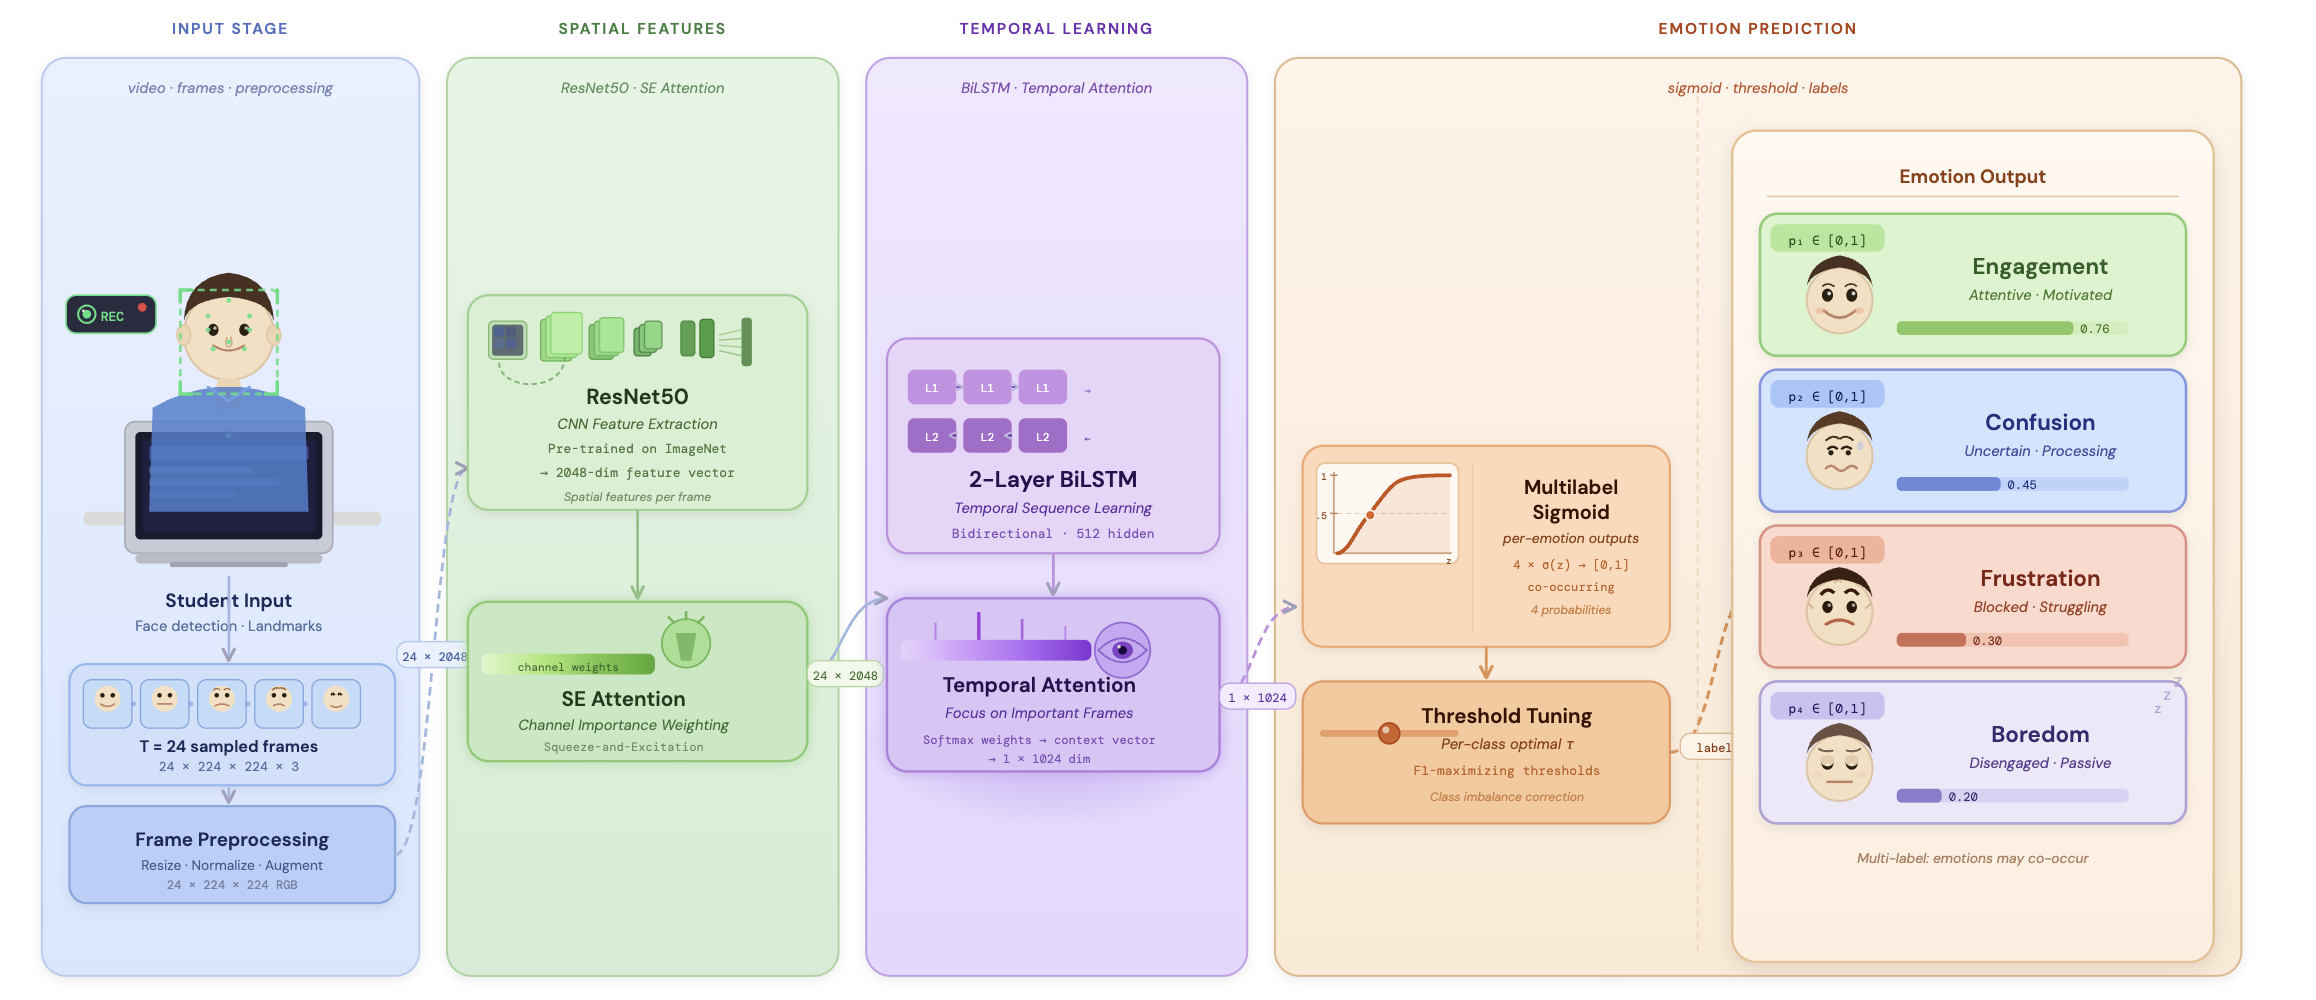
\includegraphics[width=1.25\textwidth,keepaspectratio]{Figures/fer_pipeline.png}}
    \caption{End-to-end \ac{FER} architecture for multi-label academic affect recognition. A learner video clip is sampled to a fixed length of $T = 24$ frames and preprocessed, per-frame spatial features are extracted with a ResNet-50 backbone and recalibrated by a Squeeze-and-Excitation channel-attention block, their temporal pattern is encoded by a two-layer Bidirectional \ac{LSTM}, the time steps are aggregated by a temporal attention pooling layer, and a multi-label classification head produces four independent sigmoid scores for Boredom, Engagement, Confusion, and Frustration. Per-label thresholds tuned on the validation set turn these scores into the final binary affect labels.}
    \label{fig:fer_pipeline}
\end{figure}

\subsection{Spatial Backbone: ResNet-50}\label{sec:method_resnet}

The spatial backbone is ResNet-50~\cite{he_resnet_2016}, a fifty-layer convolutional neural network with residual connections that add the input of each block back to its output. The backbone is loaded with weights pre-trained on ImageNet and is fine-tuned end-to-end. The ImageNet classification head is removed, leaving the convolutional body and the global average pooling layer. For each input frame the body produces a $2048$-dimensional feature vector. The $T = 24$ frames of a clip are passed through the backbone in a single batched call by reshaping the input to $[B \cdot T, C, H, W]$, and the resulting features are reshaped back to $[B, T, 2048]$ before the next block.

\subsection{Squeeze-and-Excitation Channel Attention}\label{sec:method_se}

The per-frame feature vectors are passed through a \ac{SE} block~\cite{hu_squeeze_2018}. The \ac{SE} block re-weights the $2048$ feature channels of each frame using two fully connected layers. The first layer projects the channel vector to a hidden size of $\max(2048 / 16, 64) = 128$ with a ReLU activation, and the second projects it back to $2048$ with a sigmoid activation, producing one importance weight per channel. The weights are multiplied element-wise onto the original feature vector. The output has the same shape $[B, T, 2048]$ as the input.

\subsection{Temporal Encoder: Two-Layer \ac{BiLSTM}}\label{sec:method_bilstm}

The recalibrated per-frame features are passed to a two-layer \ac{BiLSTM} network~\cite{hochreiter_lstm_1997}. The \ac{BiLSTM} has two stacked layers with hidden size $256$ in each direction and a dropout of $0.5$ between layers. It reads the $[B, T, 2048]$ sequence produced by the \ac{SE} block and outputs a sequence of shape $[B, T, 512]$, where $512 = 2 \cdot 256$ comes from concatenating the forward and backward hidden states at each time step.

\subsection{Temporal Attention Pooling}\label{sec:method_temporal_attention}

The temporal attention pooling layer aggregates the \ac{BiLSTM} outputs into a single clip-level vector~\cite{vaswani_attention_2017}. For each of the $T = 24$ time-step vectors, the layer computes an unnormalised attention score with a fully connected layer of hidden size $128$ and a $\tanh$ activation, followed by a second fully connected layer that produces a single scalar. The $T$ scalars are normalised by a softmax across time, and the clip representation is formed as the weighted sum of the time-step vectors with these weights. The output has shape $[B, 512]$.

\subsection{Multi-label Classification Head}\label{sec:method_head}

The clip representation is mapped to four label logits by a classification head consisting of a dropout layer, a linear projection to $256$ units, a ReLU activation, a second dropout layer, and a final linear projection to four logits. Both dropout layers use a dropout rate of $0.5$. A sigmoid activation is applied independently to each of the four logits, producing four scores in the interval $[0,1]$. The four scores correspond, in order, to Boredom, Engagement, Confusion, and Frustration~\cite{gupta_daisee_2016}. They are converted into binary predictions by the per-label thresholds described in Section~\ref{sec:method_thresholds}.

\begin{table}[H]
\centering
\small
\setlength{\tabcolsep}{4pt}
\renewcommand{\arraystretch}{1.2}
\caption{Summary of the components that constitute the proposed \ac{FER} pipeline and the supporting studies in which each component, or a close relative of it, has been reported. The first five rows correspond to the five architectural blocks described in Section~\ref{sec:method_architecture}; the last two rows correspond to the training-time loss reweighting and the decision-time threshold calibration described in Section~\ref{sec:method_training}.}
\label{tab:fer_architecture_motivation}
\begin{tabular}{>{\RaggedRight\arraybackslash}p{2.8cm}
                >{\RaggedRight\arraybackslash}p{3.0cm}
                >{\RaggedRight\arraybackslash}p{3.5cm}
                >{\RaggedRight\arraybackslash}p{5.0cm}}
\toprule
\textbf{Component} & \textbf{Supporting Studies} & \textbf{Role in the Pipeline} & \textbf{Function Reported in Prior Work} \\
\midrule
ResNet-50 &
\cite{he_resnet_2016,aly_revolutionizing_2025} &
Per-frame spatial feature extractor producing a 2048-dimensional vector &
Deep convolutional network with residual connections, pre-trained on ImageNet and adopted as a stable backbone for transfer learning in vision tasks \\

Squeeze-and-Excitation block &
\cite{hu_squeeze_2018,aly_revolutionizing_2025,liu_dynamic_2026} &
Channel attention applied to the per-frame feature vectors &
Lightweight module that recalibrates feature channels to emphasise informative responses \\

Two-layer \ac{BiLSTM} &
\cite{hochreiter_lstm_1997,tulsani_realtime_2025} &
Temporal sequence encoder operating on the recalibrated per-frame features &
Recurrent architecture that captures bidirectional temporal dependencies across video frames \\

Temporal Attention &
\cite{vaswani_attention_2017,mehta_three-dimensional_2022,su_leveraging_2024} &
Time-step weighting mechanism that aggregates the \ac{BiLSTM} outputs into a clip-level representation &
Attention layer that assigns importance scores to temporal features prior to aggregation \\

Multi-label classification head &
\cite{gupta_daisee_2016,rianto_engagement_2025} &
Four independent sigmoid outputs producing the affect vector &
Standard formulation for multi-label classification tasks in which categories may co-occur \\

\midrule

Weighted binary cross-entropy &
\cite{abedi_improving_2021,mehta_three-dimensional_2022,rianto_engagement_2025} &
Loss reweighting at the optimisation level &
Loss-level reweighting reported in the literature as a means of addressing class-frequency differences in multi-label settings \\

Per-label threshold tuning &
\cite{rianto_engagement_2025,mehta_three-dimensional_2022} &
Decision-boundary calibration on the validation set &
Validation-driven calibration of the per-label decision threshold used to convert sigmoid scores into binary predictions \\
\bottomrule
\end{tabular}
\end{table}

\section{Training and Evaluation Protocol}\label{sec:method_training}

The \ac{FER} module is trained end-to-end: both the ResNet-50 backbone and the upper temporal blocks are updated by gradient descent.

\subsection{Loss Function and Imbalance Handling}\label{sec:method_loss}

The loss function is the per-label binary cross-entropy with logits (\texttt{BCEWithLogitsLoss}), with a positive-class weight per label. The four labels are treated as independent binary decisions and the per-label losses are summed across the batch.

The class-frequency differences described in Section~\ref{sec:method_dataset} are handled at three complementary levels of the training pipeline. First, at the \textbf{data level}, the dominant-group resampling step defined in Section~\ref{sec:method_oversampling} duplicates training clips so that minority dominant categories are seen more often by the model during each epoch. Second, at the \textbf{loss level}, a per-label positive-class weight is incorporated into the binary cross-entropy loss. For each label, the weight is derived from the ratio of negative to positive training examples and is bounded to a predefined range to prevent extremely rare labels from dominating the optimisation process. This increases the penalty for misclassified positive examples on minority labels while maintaining stable gradients during training. Third, at the \textbf{decision level}, a per-label decision threshold is tuned on the validation set as described in Section~\ref{sec:method_thresholds}, so that the conversion from sigmoid score to binary prediction is calibrated separately for each of the four affective labels.

\subsection{Optimisation}\label{sec:method_optim}

The model is optimised with AdamW. The learning rate is set to $5 \times 10^{-5}$, the weight-decay coefficient to $10^{-5}$, and the batch size to $4$. Gradients are clipped at a maximum global norm of $5.0$. A learning-rate scheduler of type \texttt{ReduceLROnPlateau} monitors the validation Macro F1 score; if the metric does not improve for two consecutive validation rounds, the learning rate is multiplied by $0.5$. The model is trained for up to twelve epochs, with an early-stopping rule that interrupts training if the validation Macro F1 does not improve for four epochs in a row. The checkpoint with the highest validation Macro F1 is retained.

\subsection{Per-Label Threshold Tuning}\label{sec:method_thresholds}

The \ac{FER} model produces a continuous sigmoid score in $[0,1]$ for each of the four affective labels. Converting these scores into binary predictions requires a decision threshold per label. A single global threshold of $0.5$ is not optimal for this task because the \ac{DAiSEE} dataset is class-imbalanced and because each affective state exhibits a different score distribution; a uniform threshold therefore yields uneven performance across labels. Label-specific thresholds are consequently calibrated independently on the validation set.

After every training epoch, the current model is applied to the full validation set, producing a probability matrix of size $N_{\mathrm{val}} \times 4$. For each label, a range of candidate thresholds between $0.10$ and $0.70$ is evaluated, and the threshold that achieves the highest validation F1 score is selected. The four label-specific thresholds chosen at the best-performing validation checkpoint are retained and applied at test time. This calibration step constitutes the final decision stage of the \ac{FER} pipeline, converting sigmoid probability estimates into the binary affect predictions consumed by the adaptive tutoring module.

\subsection{Evaluation Metrics}\label{sec:method_metrics}

The \ac{FER} module is evaluated using a set of multi-label classification metrics, all computed at the per-label decision thresholds calibrated in Section~\ref{sec:method_thresholds}. The following notation is used throughout this section. For a given affective label, a \emph{True Positive} (TP) is a clip correctly predicted as positive; a \emph{True Negative} (TN) is a clip correctly predicted as negative; a \emph{False Positive} (FP) is a clip incorrectly predicted as positive when the ground-truth label is negative; and a \emph{False Negative} (FN) is a clip incorrectly predicted as negative when the ground-truth label is positive. Let $L = 4$ denote the number of affective labels and $N$ the number of clips in the evaluation set. Every metric defined below is computed during both validation and final test evaluation, and every metric is reported in the experimental results of Chapter~\ref{chap:results}.

\paragraph{Per-label Accuracy.}
Per-label accuracy measures the proportion of all predictions for a given label, both positive and negative,that are classified correctly \cite{gothwal_vibed-net_2025}:
\begin{equation}
\left[\; \mathrm{Accuracy}_{\ell} \;=\; \frac{\mathrm{TP}_{\ell} + \mathrm{TN}_{\ell}}{\mathrm{TP}_{\ell} + \mathrm{TN}_{\ell} + \mathrm{FP}_{\ell} + \mathrm{FN}_{\ell}} \;\right].
\label{eq:accuracy}
\end{equation}
Per-label accuracy is reported individually for each of the four affective states. Because the dataset is heavily imbalanced, a high per-label accuracy can be achieved by a model that predicts predominantly the negative class; per-label accuracy is therefore interpreted alongside F1 metrics rather than in isolation.


\paragraph{Precision.}
Precision measures the proportion of positive predictions that are genuinely positive. It quantifies how reliably the model identifies the presence of an affective state without raising false alarms \cite{gothwal_vibed-net_2025}
\begin{equation}
\left[\; \mathrm{Precision} \;=\; \frac{\mathrm{TP}}{\mathrm{TP} + \mathrm{FP}} \;\right].
\label{eq:precision}
\end{equation}

\paragraph{Recall.}
Recall measures the proportion of truly positive instances that the model successfully detects. It reflects the model's sensitivity to the presence of each affective state \cite{gothwal_vibed-net_2025}:
\begin{equation}
\left[\; \mathrm{Recall} \;=\; \frac{\mathrm{TP}}{\mathrm{TP} + \mathrm{FN}} \;\right].
\label{eq:recall}
\end{equation}
A high recall indicates that the model misses few genuine cases, which is particularly important for minority affective states such as Confusion and Frustration in the \ac{DAiSEE} dataset.

\paragraph{F1 Score.}
The F1 score is the harmonic mean of Precision and Recall. It provides a single balanced measure that penalises both false positives and false negatives, making it well-suited for evaluation under imbalanced label distributions \cite{gothwal_vibed-net_2025}:
\begin{equation}
\left[\; \mathrm{F1} \;=\; \frac{2 \times \mathrm{Precision} \times \mathrm{Recall}}{\mathrm{Precision} + \mathrm{Recall}} \;\right].
\label{eq:f1}
\end{equation}
Per-label F1 scores are reported individually for each affective state. They are also used during per-label threshold tuning on the validation set: for each label, the threshold that maximises the per-label F1 is selected.
\paragraph{Macro F1.}
Macro F1 is computed as the unweighted mean of the per-class F1 scores, treating all classes equally regardless of their frequency. This makes it sensitive to performance on minority classes. \cite{scikit_learn}

\paragraph{Micro F1.}
Micro F1 aggregates true positives, false positives, and false negatives across all classes before computing a single F1 score. It therefore reflects overall performance weighted by the total number of samples. \cite{scikit_learn}

\paragraph{Weighted F1.}
Weighted F1 computes the average of per-class F1 scores weighted by the number of true instances in each class, providing a balance between Macro F1 and class-frequency bias. \cite{scikit_learn}

\paragraph{Samples F1.}
Samples F1 is commonly used in multi-label classification and computes the F1 score per sample by comparing the set of true labels and predicted labels, then averaging across all samples. \cite{tsoumakas2007multi, scikit_learn}
\subsection{Implementation Details}\label{sec:method_impl}

The \ac{FER} module is implemented in Python with PyTorch and torchvision. Frame input/output uses OpenCV, and metrics are computed with scikit-learn. The dataset, model, training, and evaluation scripts are organised as separate self-contained modules. The frame extraction step and the construction of the resampled training CSV are executed once offline. Training and evaluation were run on a single NVIDIA Tesla T4 GPU on the Kaggle Notebooks platform. The full set of training hyperparameters is summarised in Table~\ref{tab:fer_hparams}.

\begin{table}[H]
\centering
\caption{\ac{FER} training hyperparameters.}
\label{tab:fer_hparams}
\begin{tabular}{ll}
\toprule
\textbf{Hyperparameter} & \textbf{Value} \\
\midrule
Image size                      & $224 \times 224$ \\
Frames per clip $T$             & $24$ \\
Backbone                        & ResNet-50, ImageNet pre-trained, fine-tuned \\
\ac{SE} reduction ratio              & $16$ \\
\ac{BiLSTM} layers                   & $2$ \\
\ac{BiLSTM} hidden size              & $256$ per direction \\
Temporal attention hidden size  & $128$ \\
Classifier hidden size          & $256$ \\
Dropout                         & $0.5$ \\
Loss                            & \ac{BCE} with logits, per-label \texttt{pos\_weight} clipped to $[0.5, 6.0]$ \\
Optimiser                       & AdamW (\texttt{lr}\,$=5\!\times\!10^{-5}$, \texttt{weight\_decay}\,$=10^{-5}$) \\
Gradient clipping               & global norm $\leq 5.0$ \\
LR scheduler                    & \texttt{ReduceLROnPlateau} on val.\ Macro F1 (factor $0.5$, patience $2$) \\
Batch size                      & $4$ \\
Epochs                          & up to $12$, early stop patience $4$ on val.\ Macro F1 \\
Threshold grid                  & $0.10, 0.15, \dots, 0.70$ per label, per-label F1 max \\
Train-time augmentation         & flip $0.5$, brightness/contrast $0.5$, rotation $0.25$, blur $0.15$, crop $0.25$ \\
Oversampling multipliers        & engagement $\times 1$, boredom $\times 2$, confusion $\times 3$, frustration $\times 4$ \\
\bottomrule
\end{tabular}
\end{table}
\section{Adaptive Tutoring via Reinforcement Learning (\ac{DQN}-Based)}\label{sec:method_rl_chapter}

\subsection{Theoretical Foundations and Citation Mapping}\label{sec:method_rl_intro}

This section documents the theoretical foundations of the proposed tutoring environment. All cognitive, affective, and pedagogical mechanisms are inherited from published sources; the \ac{DQN} agent learns only to act within this theory-grounded environment. No new cognitive or affective model is proposed.

The theoretical framework is presented in two layers. Table~\ref{tab:rl_foundations} provides a conceptual overview of the modelling decisions and their motivating sources. Tables~\ref{tab:rl_operationalized} and~\ref{tab:rl_operationalized_b} form a traceability matrix in which each row states one inherited mechanism, presents its core formal rule, and cites the originating source. Part A covers the cognitive model, affective dynamics, and emotion taxonomy. Part B covers the pedagogical interventions, reward function, partial observability, and the \ac{DQN} learning algorithm. Every equation and transition rule introduced in the following subsections is traceable to a row in one of these two tables.

\renewcommand{\arraystretch}{1.5}
\begin{table}[H]
\centering
\caption{Layer 1 -- Conceptual Foundations. Each row identifies one theoretical idea that motivates a modelling decision. No equations or implementation details appear in this layer.}
\label{tab:rl_foundations}
\begin{tabular}{>{\raggedright\arraybackslash}p{5.0cm}>{\raggedright\arraybackslash}p{5.8cm}>{\raggedright\arraybackslash}p{2.8cm}}
\toprule
\textbf{Modelling Aspect} & \textbf{Theoretical Contribution} & \textbf{Primary Source} \\
\midrule
Cognitive Learning Dynamics
    & Mastery evolves through saturating learning with diminishing gains near proficiency.
    & Guzm{\'a}n \& Cruz-Mercado~\cite{guzman_developing_2025} \\
Affective State Modelling
    & Academic emotions persist over time rather than resetting after each interaction.
    & Henke et al.~\cite{henke_dsem_2026} \\
Cognitive-Affective Coupling
    & Cognitive outcomes and affective states are mutually dependent and should be modelled jointly.
    & Wang~\cite{wang_factored_pomdp_2018} \\
Academic Emotion Taxonomy
    & Four discrete academic emotions govern learning behaviour and motivational states.
    & Pekrun~\cite{pekrun_control-value_2006} \\
Challenge-Skill Balance
    & Optimal learning occurs within a moderate difficulty band; mismatches drive negative affect.
    & Csikszentmihalyi~\cite{csikszentmihalyi_flow_1990} \\
Multi-Objective Reward Design
    & Tutoring rewards should reflect both learning progress and affective well-being simultaneously.
    & Kong et al.~\cite{kong_real-time_2025} \\
Utility Aggregation
    & Cognitive and affective objectives should be combined into a single unified optimisation target.
    & Hern{\'a}ndez et al.~\cite{hernandez_affective_2015} \\
Partial Observability
    & Tutoring agents operate without direct access to latent task parameters.
    & Ramachandran et al.~\cite{ramachandran_pomdp_2018} \\
\bottomrule
\end{tabular}
\end{table}

% -----------------------------------------------------------------------
% Table 4.4 Part A — Cognitive model, affective dynamics, emotion taxonomy
% -----------------------------------------------------------------------
\renewcommand{\arraystretch}{1.7}
\begin{table}[H]
\centering
\small
\caption{Layer 2 -- Theory-to-Methodology Traceability (Part A: Cognitive Model and Affective State Structure). Each row states one inherited mechanism, its core formal rule, and the originating source. Specific coefficient values and hyperparameter settings appear in the body text. Part B (Table~\ref{tab:rl_operationalized_b}) and Part C (Table~\ref{tab:rl_operationalized_c}) follow.}
\label{tab:rl_operationalized}
\begin{tabular}{>{\raggedright\arraybackslash}p{2.4cm}
                >{\raggedright\arraybackslash}p{5.0cm}
                >{\raggedright\arraybackslash}p{4.0cm}
                >{\raggedright\arraybackslash}p{2.2cm}}
\toprule
\textbf{Component} & \textbf{Methodological Rule} & \textbf{Formal Rule} & \textbf{Source} \\
\midrule
\multicolumn{4}{@{\hspace{0.3em}}l}{\small\bfseries Cognitive Model} \\
\midrule

Item correctness
    & Computes response correctness from the difference between learner mastery and task difficulty.
    & $\Pr(\text{correct}) = \sigma\!\bigl(\beta(k - \alpha d)\bigr)$
    & Guzm{\'a}n \& Cruz-Mercado \cite{guzman_developing_2025} \\[0.4em]

Mastery update
    & Mastery grows toward saturation, with stronger updates after incorrect responses than correct ones.
    & $k_{t+1} = \mathrm{clip}\!\bigl(k_t + g_t(1{-}k_t) - \delta_t\bigr)$
    & Guzm{\'a}n \& Cruz-Mercado \cite{guzman_developing_2025} \\

\midrule
\multicolumn{4}{@{\hspace{0.3em}}l}{\small\bfseries Affective State Structure} \\
\midrule

Factored learner state
    & Represents cognition and affect as separate components within a single learner state.
    & $\mathbf{s}_t = (k_t,\, e_t,\, f_t,\, c_t,\, b_t,\, \iota_t)$
    & Wang \cite{wang_factored_pomdp_2018} \\[0.4em]

Cognitive--affective coupling
    & Affect evolves based on emotion, action, and mastery state..
    & $P(e' \mid e,\, a,\, d')$
    & Wang \cite{wang_factored_pomdp_2018} \\

\bottomrule
\end{tabular}
\end{table}

% -----------------------------------------------------------------------
% Table 4.4 Part B — Affective dynamics cont., mismatch, emotion, interventions, reward
% -----------------------------------------------------------------------
\renewcommand{\arraystretch}{1.7}
\begin{table}[H]
\centering
\small
\caption{Layer 2 -- Theory-to-Methodology Traceability (Part B: Affective Dynamics, Challenge--Skill Mismatch, Emotion Taxonomy, Pedagogical Interventions, and Reward Function). Continuation of Table~\ref{tab:rl_operationalized} (Part A); Part C (Table~\ref{tab:rl_operationalized_c}) follows.}
\label{tab:rl_operationalized_b}
\begin{tabular}{>{\raggedright\arraybackslash}p{2.4cm}
                >{\raggedright\arraybackslash}p{5.0cm}
                >{\raggedright\arraybackslash}p{4.0cm}
                >{\raggedright\arraybackslash}p{2.2cm}}
\toprule
\textbf{Component} & \textbf{Methodological Rule} & \textbf{Formal Rule} & \textbf{Source} \\
\midrule
\multicolumn{4}{@{\hspace{0.3em}}l}{\small\bfseries Affective Dynamics} \\
\midrule

Affective AR(1) dynamics
    & Affect changes gradually toward targets influenced by action and task–skill mismatch.
    & $x_{t+1} = \lambda_x x_t + (1{-}\lambda_x)\,\tau_x(a_t, m_t) + \varepsilon_t$
    & Henke et al. \cite{henke_dsem_2026} \\

\midrule
\multicolumn{4}{@{\hspace{0.3em}}l}{\small\bfseries Challenge--Skill Mismatch} \\
\midrule

Mismatch regimes
    & Task–mastery gap defines whether the task is too hard, too easy, or in the flow zone, shaping affective responses.
    & $m_t = d_t - k_t$;\newline $m_t \gg 0 \Rightarrow$ hard;\newline $m_t \ll 0 \Rightarrow$ easy;\newline $m_t \approx 0 \Rightarrow$ flow
    & Csikszentmihalyi \cite{csikszentmihalyi_flow_1990} \\

\midrule
\multicolumn{4}{@{\hspace{0.3em}}l}{\small\bfseries Emotion Taxonomy and Discretisation} \\
\midrule

Discrete emotion rule
    & Maps affect to four discrete emotion classes through thresholding.
    & $\iota_t \leftarrow \text{priority}(f_t, c_t, b_t)$ $\to \{\text{frustrated},$ $\text{confused, bored,}$ $\text{engaged}\}$
    & Pekrun \cite{pekrun_control-value_2006} \\

\midrule
\multicolumn{4}{@{\hspace{0.3em}}l}{\small\bfseries Pedagogical Interventions} \\
\midrule

Action set and affective targets
    & Each intervention specifies how it modifies affective targets based on pedagogical theory.
    & $\mathcal{A} = \{$hint, scaffold, encouragement, simplify, harder, break, explanation, no-action$\}$;\newline each $a$ defines $\tau_x^{\mathrm{act}}(a)$
    & Sudharsan et al. \cite{sudharsan_intervention_2026} \\

\midrule
\multicolumn{4}{@{\hspace{0.3em}}l}{\small\bfseries Reward Function} \\
\midrule

Normalised learning gain
    & Measures progress as normalized gain in mastery.
    & $\Delta k_{\mathrm{norm}} = \dfrac{k_{t+1} - k_t}{1 - k_t}$
    & Hake \cite{hake_normalized_gain_1998} \\[0.4em]

Multi-objective reward
    & Uses a single reward combining learning progress with affective regulation signals.
    & $r_t = w_k\,\Delta k_{\mathrm{norm}} + w_e\,e_t - w_f\,f_t - w_b\,b_t - w_c\,c_t$
    & Kong et al. \cite{kong_real-time_2025} \\

\bottomrule
\end{tabular}
\end{table}

% -----------------------------------------------------------------------
% Table 4.4 Part C — Partial observability and \ac{DQN} learning algorithm
% -----------------------------------------------------------------------
\renewcommand{\arraystretch}{1.7}
\begin{table}[H]
\centering
\small
\caption{Layer 2 -- Theory-to-Methodology Traceability (Part C: Partial Observability, Episode Termination, and \ac{DQN} Learning Algorithm). Continuation of Table~\ref{tab:rl_operationalized} (Part A) and Table~\ref{tab:rl_operationalized_b} (Part B), completing the traceability matrix.}
\label{tab:rl_operationalized_c}
\begin{tabular}{>{\raggedright\arraybackslash}p{2.4cm}
                >{\raggedright\arraybackslash}p{5.0cm}
                >{\raggedright\arraybackslash}p{4.0cm}
                >{\raggedright\arraybackslash}p{2.2cm}}
\toprule
\textbf{Component} & \textbf{Methodological Rule} & \textbf{Formal Rule} & \textbf{Source} \\
\midrule
\multicolumn{4}{@{\hspace{0.3em}}l}{\small\bfseries Partial Observability and Episode Termination} \\
\midrule

Hidden task difficulty
    & Task difficulty is hidden from the agent, consistent with a \ac{POMDP} tutoring setting.
    & $\mathbf{o}_t = (k_t, e_t, f_t, c_t, b_t, \iota_t)$;\newline $d_t \notin \mathbf{o}_t$
    & Ramachandran et al. \cite{ramachandran_pomdp_2018} \\[0.4em]

Dropout termination
    & Episode ends when sustained frustration exceeds a dropout threshold, representing learner disengagement..
    & $\phi_t = 1$ sustained for ${\geq}\,T_{\text{drop}}$ steps $\Rightarrow$ episode terminated
    & Ramachandran et al. \cite{ramachandran_pomdp_2018} \\

\midrule
\multicolumn{4}{@{\hspace{0.3em}}l}{\small\bfseries \ac{DQN} Learning Algorithm} \\
\midrule

\ac{DQN} optimisation
    & The Q-network is trained by minimizing the difference between its predictions and stable targets generated by a frozen copy of the network, using sampled past experiences for stable learning.
    & $y_t = r_t + \gamma\,\max_{a'} Q^-\!(\mathbf{s}_{t+1}, a';\,\theta^-)$;\newline $L(\theta) = \mathbb{E}_{\mathcal{B}}\!\bigl[\mathrm{smoothL_1}(y_t - Q(\mathbf{s}_t, a_t;\theta))\bigr]$
    & Mnih et al. \cite{mnih_dqn_2015};\newline Raffin et al. \cite{raffin_sb3_2021} \\

\bottomrule
\end{tabular}
\end{table}
\renewcommand{\arraystretch}{1}
The block diagram of Figure~\ref{fig:dqn_mdp} renders the learner state as $\mathbf{s}_t = [k_t, e_t]$ for visual compactness. In the formal model, the symbol $e_t$ expands into the four affective scalars and the discrete academic-emotion identifier defined in Equation~\eqref{eq:student_state}. The resulting formulation is consistent with established affective tutoring architectures in the literature~\cite{wang_factored_pomdp_2018,guzman_developing_2025,kong_real-time_2025}.

\subsection{System Architecture and Reinforcement Learning Formulation}\label{sec:method_rl_architecture}

The learning environment is formalised as a discrete-time Markov decision process. Student and tutor interactions are modelled through learner observations, pedagogical actions, and stochastic transitions over a cognitive and affective state.

At each decision step $t$, the environment emits an observation $\mathbf{o}_t$ and an admissibility mask $\mathbf{m}_t \in \{0,1\}^{|\mathcal{A}|}$ that encodes pedagogical safety constraints. The \ac{DQN} policy then selects an admissible action $a_t$. The learner state evolves from $\mathbf{s}_t$ to $\mathbf{s}_{t+1}$ under the transition kernel of Sections~\ref{sec:method_mdp} and~\ref{sec:method_emotion_engagement}. Finally, a scalar reward $r_t$ is returned by the multi-objective formulation of Section~\ref{sec:method_reward}.

Episodes terminate under three conditions: task completion when mastery exceeds a fixed threshold, persistent negative affect indicating learner disengagement, or reaching the maximum interaction horizon.

\begin{figure}[H]
    \centering
    \makebox[\textwidth][c]{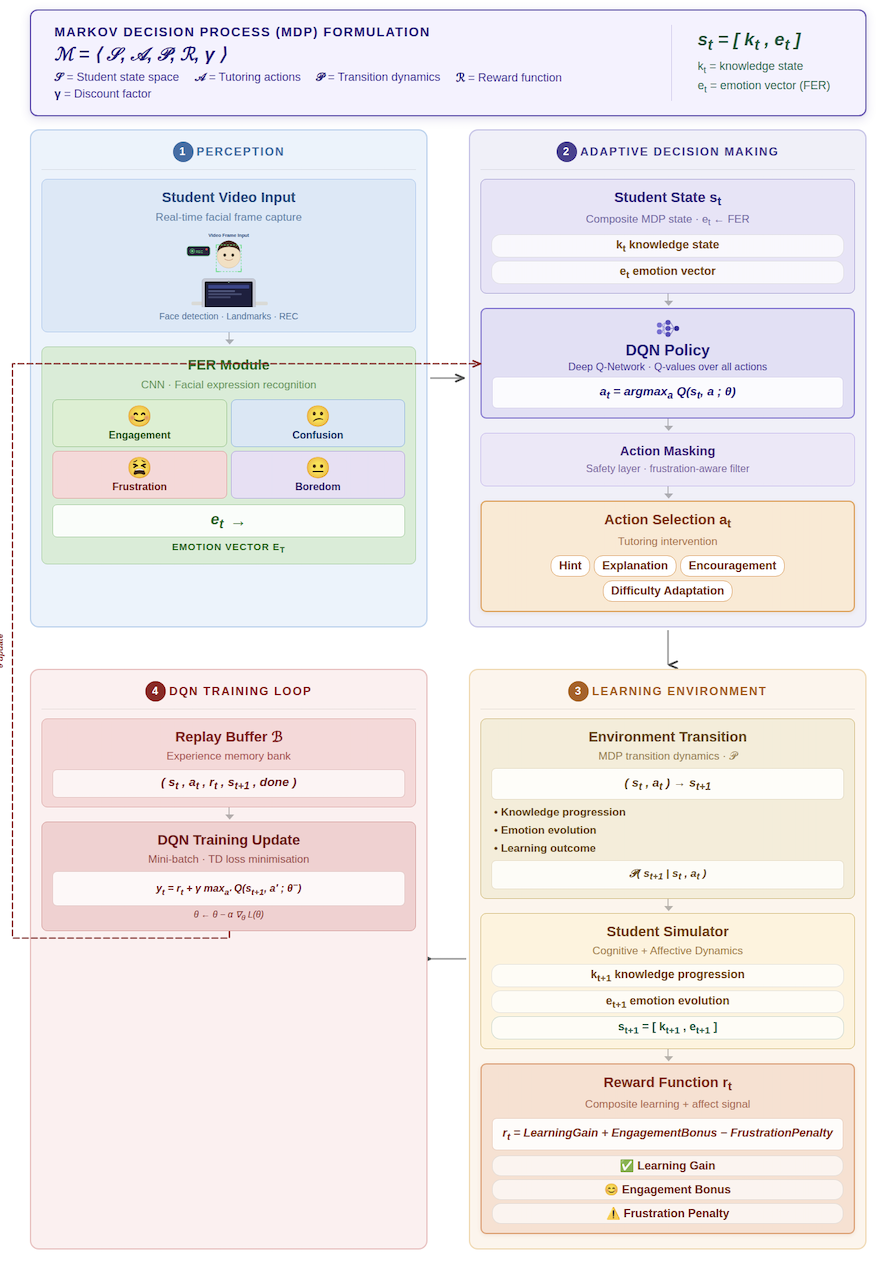
\includegraphics[width=1\textwidth,keepaspectratio]{Figures/final.png}}
    \caption{End-to-end \ac{DQN}-based adaptive tutoring framework. The perception module contributes affective information to the state representation, the \ac{DQN} selects tutoring actions, and the environment provides rewards and state transitions for replay-based learning. For clarity, the state is depicted as $\mathbf{s}_t=[k_t,e_t]$, where $e_t$ denotes the affective components of Equation~\eqref{eq:student_state}.}
    \label{fig:dqn_mdp}
\end{figure}

The system is structured as a reinforcement learning architecture consisting of interacting cognitive, affective, and policy components. A synthetic student simulator supplies the cognitive and affective dynamics. A Markov-decision-process environment orchestrates the transition kernel. An affective interface produces the discrete academic-emotion identifier. A reward formulation combines cognitive gain with affective regulation. A \ac{DQN} agent learns the policy. An evaluation pipeline aggregates outcomes across episodes and seeds.

Training is performed offline against a synthetic population, consistent with prior reinforcement-learning-based tutoring simulations~\cite{guzman_developing_2025,kong_real-time_2025}. The real-time facial-expression-recognition pipeline of Section~\ref{sec:method_architecture} is treated as a modular extension that can replace the synthetic affective channel at deployment. It is not activated in the reported experimental setting.\label{sec:method_rl_formulation}

\subsection{Markov Decision Process and Environment Model}\label{sec:method_rl_mdp_parent}

This section formally defines the Markov decision process underlying the adaptive tutoring system and specifies the models that govern cognitive state evolution, affective dynamics, learner heterogeneity, task structure, observation, pedagogical actions, and reward. Together these components constitute the theory-inherited environment within which the \ac{DQN} policy is trained.

\subsubsection{State Space and Cognitive Model}\label{sec:method_mdp}

The tutoring task is formalised as a Markov decision process $\mathcal{M} = (\mathcal{S}, \mathcal{A}, P, R, \gamma)$ with discount factor $\gamma = 0.99$~ following standard practice in deep reinforcement learning and serves as a design hyperparameter controlling the emphasis on long-term rewards \cite{mnih_dqn_2015}. Following the factored intelligent-tutoring \ac{POMDP} of Wang~\cite{wang_factored_pomdp_2018} and the partial-observability framing of Ramachandran et al.~\cite{ramachandran_pomdp_2018}, the latent learner state combines one cognitive component, four continuous affective dimensions, and one categorical academic-emotion identifier:
\begin{equation}
    \mathbf{s}_t = \bigl(k_t,\; e^\mathrm{eng}_t,\; f_t,\; c_t,\; b_t,\; \iota_t\bigr) \in [0,1]^5 \times \{0,1,2,3\},
    \label{eq:student_state}
\end{equation}
where $k_t$ is the scalar mastery, $e^\mathrm{eng}_t$ engagement, $f_t$ frustration, $c_t$ confusion, $b_t$ boredom, and $\iota_t$ the academic-emotion identifier defined over the four-class taxonomy of Pekrun~\cite{pekrun_control-value_2006}.

A single scalar mastery variable $k_t \in [0,1]$ governs the cognitive state evolution. No auxiliary skill vector or item-level knowledge component is modelled. An internal latent task difficulty $d_t \in [0,1]$ is maintained by the environment but is not exposed to the policy, in line with the partial-observability assumption of Ramachandran et al.~\cite{ramachandran_pomdp_2018}. The observation accessible to the agent is therefore a projection of $\mathbf{s}_t$ together with an optional affective-persistence channel introduced in Section~\ref{sec:method_gymnasium}.

The cognitive component follows the saturating learning model of Guzm{\'a}n \& Cruz-Mercado~\cite{guzman_developing_2025}. The probability of a correct response on an item of difficulty $d$ by a learner of mastery $k$ is modelled by a logistic function of their difference:
\begin{equation}
    \Pr(\text{correct} \mid k, d) = \sigma\!\bigl(\beta\, (k - \alpha\, d)\bigr),
    \label{eq:irt}
\end{equation}
with discrimination $\beta = 3.0$ and difficulty scale $\alpha = 1.0$.

Mastery itself evolves by a saturating update on the remaining headroom $(1 - k_t)$, scaled by a learning gain $g_t$ that depends on the chosen pedagogical action and on the learner's personality, together with a forgetting correction and Gaussian noise. The core learning rule is
\begin{equation}
    k_{t+1} = \mathrm{clip}_{[0,1]}\!\bigl( k_t + g_t\,(1 - k_t) - \delta_t + \eta_t \bigr).
    \label{eq:knowledge_update}
\end{equation}
The learning gain is defined as $g_t = g_\mathrm{base}(a_t)\,\gamma_s\,\kappa(\text{correctness}_t)$, where $g_\mathrm{base}(a_t)$ is the base increment associated with action $a_t$, $\gamma_s$ is the personality-level learning rate, and $\kappa$ is a multiplicative factor that depends on whether the learner's response was correct. The forgetting term $\delta_t$ subtracts a small fraction of mastery when the response is incorrect or when engagement falls below $0.3$, capturing the disengagement-driven decay reported in the academic-emotion literature~\cite{pekrun_control-value_2006}. The noise term $\eta_t \sim \mathcal{N}(0,\, 0.02^2)$ models residual stochasticity.

The per-learner parameters $(\gamma_s, \beta_s, \lambda_s, \rho_s)$ scale, respectively, the learning rate, the sensitivity to challenge and skill mismatch, the forgetting rate, and the patience. Their population-level sampling distributions are specified in Section~\ref{sec:method_synthetic_student}.

\subsubsection{Affective State Dynamics}\label{sec:method_emotion_engagement}

The affective dynamics are constructed in five conceptual steps and operationalised by Equation~\eqref{eq:ar1_affect} below.

\textbf{Step 1: cognitive update.} The mastery update of Equation~\eqref{eq:knowledge_update} produces an updated mastery $k_{t+1}$, which subsequently shapes the challenge and skill mismatch entering the affective targets.

\textbf{Step 2: emotional persistence.} Each continuous affective dimension $x \in \{e^\mathrm{eng}, f, c, b\}$ retains a fraction $\lambda_x$ of its previous value, following the first-order autoregressive account of academic affect of Henke et al.~\cite{henke_dsem_2026}. The empirically derived persistence coefficients are $\lambda_f = 0.69$, $\lambda_e = 0.60$, $\lambda_c = 0.47$, and $\lambda_b = 0.36$.

\textbf{Step 3: mismatch effect.} The challenge and skill mismatch $m_t = d_t - k_{t+1}$ drives a baseline target $\tau_x^{\mathrm{mm}}$ for each affective dimension. When $m_t > 0.3$, the task is too hard and the targets push frustration and confusion upward. When $m_t < -0.3$, the task is too easy and the boredom target rises. Within the band $|m_t| \leq 0.3$, the targets fall in a moderate-engagement regime consistent with the flow-zone construct of Csikszentmihalyi~\cite{csikszentmihalyi_flow_1990}.

\textbf{Step 4: intervention modulation.} The chosen pedagogical action $a_t$ may override selected target dimensions with action-specific values $\tau_x^{\mathrm{act}}(a_t)$, following the intervention catalogue of Sudharsan et al.~\cite{sudharsan_intervention_2026}. For example, hints lower the confusion target, encouragement lowers the frustration target, and breaks raise the engagement target.

\textbf{Step 5: final state composition.} The effective target combines the mismatch baseline and the intervention overrides into a single value $\tau_x(a_t, m_t)$. Each affective dimension is then updated by
\begin{equation}
    x_{t+1} = \mathrm{clip}_{[0,1]}\!\bigl( \lambda_x\, x_t + (1 - \lambda_x)\, \tau_x(a_t, m_t) + \varepsilon_t \bigr), \qquad \varepsilon_t \sim \mathcal{N}(0,\, 0.03^2).
    \label{eq:ar1_affect}
\end{equation}
Combined with the mastery update of Equation~\eqref{eq:knowledge_update}, this composition realises the factored cognitive and affective transition $P(e' \mid e, a, d')$ proposed by Wang~\cite{wang_factored_pomdp_2018}.

\paragraph{Emotion taxonomy and two separate thresholding rules.}
The categorical academic-emotion identifier $\iota \in \{\text{confused}, \text{bored}, \text{frustrated}, \text{engaged}\}$ adopts Pekrun's four-class taxonomy~\cite{pekrun_control-value_2006}. Two thresholding rules govern $\iota$. These two mechanisms operate in separate pipelines and must not be conflated.

\textit{Rule A: synthetic emotion discretisation.} In the synthetic-training regime, the continuous affective scalars are mapped to a discrete class by a priority rule applied to their intensities. The label \emph{frustrated} is assigned when $f > 0.6$, \emph{confused} when $c > 0.5$, \emph{bored} when $b > 0.5$, and \emph{engaged} otherwise. These intensity thresholds were not chosen arbitrarily but calibrated empirically on validation rollouts to maximise cumulative reward and stabilise learning dynamics.

\textit{Rule B: facial-expression-recognition confidence filtering.} When the real-time facial-expression-recognition pipeline of Section~\ref{sec:method_architecture} replaces the synthetic affective channel, a predicted emotion label is accepted only when the network's predicted probability exceeds a confidence threshold of $0.5$. If the confidence falls below this threshold, the previously emitted emotion is retained. This confidence threshold was likewise selected through empirical tuning on validation experiments, balancing label responsiveness against noise-induced policy instability.

Although the two rules share the numerical value $0.5$, they apply to different quantities. Rule A thresholds affective intensities. Rule B thresholds classifier confidences. The two rules never coexist within a single inference path.

\subsubsection{Synthetic Student Population}\label{sec:method_synthetic_student}

Training is performed against a fixed population of $N = 10{,}000$ synthetic learners. This sample size is consistent with prior reinforcement-learning tutoring simulations~\cite{guzman_developing_2025,kong_real-time_2025,ramachandran_pomdp_2018} and is chosen to ensure statistical stability of aggregate metrics across seeds and learner heterogeneity.

Each synthetic learner is parameterised by nine heterogeneity coefficients drawn independently from uniform distributions, covering the personality parameters $(\gamma_s, \beta_s, \lambda_s, \rho_s)$ of Section~\ref{sec:method_mdp} together with auxiliary traits of frustration tolerance, boredom sensitivity, engagement recovery, baseline confidence, and persistence. For reporting purposes only, each learner is post-hoc classified into one of four illustrative types (fast learner, slow learner, easily frustrated, patient); this classification has no effect on transition dynamics.

At the start of each tutoring episode, the initial learner state is sampled from learner-specific uniform ranges over $k_0$, $e_0^\mathrm{eng}$, $f_0$, $c_0$, and $b_0$, the initial academic-emotion identifier is set to \emph{engaged}, and the latent task difficulty $d_0$ is drawn from a uniform range. The difficulty is subsequently modified only through the two difficulty-adjusting interventions defined in Section~\ref{sec:method_action_space} and remains hidden from the policy, in accordance with the partial-observability assumption of Ramachandran et al.~\cite{ramachandran_pomdp_2018}.

\subsubsection{Observation, Transition, and Termination}\label{sec:method_gymnasium}

\paragraph{State definition.} The latent learner state $\mathbf{s}_t$ defined in Equation~\eqref{eq:student_state} carries the scalar mastery, the four continuous affective scalars, and the categorical academic-emotion identifier. The latent task difficulty $d_t$ is internal to the environment and is updated only through the difficulty-adjusting interventions of Section~\ref{sec:method_action_space}.

\paragraph{Observation model.} The observation vector emitted to the policy is the projection of $\mathbf{s}_t$ onto the channels visible to the agent:
\begin{equation}
    \mathbf{o}_t^{(6)} = \bigl(k_t,\; e^\mathrm{eng}_t,\; f_t,\; c_t,\; b_t,\; \iota_t\bigr)^\top.
    \label{eq:obs_v6}
\end{equation}\label{sec:method_observation}
When the affective-persistence channel is enabled, the observation is extended with an additional feature that measures how long frustration has been continuously active. This value is computed from the number of consecutive steps with active frustration, normalised and clipped to the range $[0,1]$. Channel-masking ablations then set individual observation components to zero to evaluate their contribution without retraining the model.


\paragraph{Transition function.}
The state transition $P(\mathbf{s}_{t+1} \mid \mathbf{s}_t, a_t)$ is built from four steps: response correctness, mastery update, affect update, and emotion classification. First, student responses are generated using the logistic correctness model in Equation~\eqref{eq:irt}. Next, learner mastery is updated using the rule in Equation~\eqref{eq:knowledge_update}. Affective states are then updated gradually using the autoregressive model in Equation~\eqref{eq:ar1_affect}. Finally, continuous affect is mapped to discrete emotion classes as described in Section~\ref{sec:method_emotion_engagement}.

In addition, the environment tracks a persistent-frustration flag $\phi_t \in \{0,1\}$, which becomes active when frustration remains above $0.7$ for three consecutive steps and is reset when it drops below $0.5$.

\paragraph{Episode termination.} Episodes terminate under three conditions. The first condition is task completion, triggered when $k_{t+1} \geq 0.95$. The second condition is a learner-dropout event, triggered when $\phi_t$ remains active for at least five consecutive interaction steps and treated as a dropout signal in the sense of Ramachandran et al.~\cite{ramachandran_pomdp_2018}. The third condition is the maximum interaction horizon, reached when the episode length attains fifty interaction steps.

\subsubsection{Reward Function}\label{sec:method_reward}

The reward function is operationalised as a multi-objective scalar that combines cognitive gain with affective regulation, following the formulation of Kong et al.~\cite{kong_real-time_2025}. The theoretical motivation for jointly optimising cognitive and affective objectives is discussed in Section~\ref{sec:method_rl_intro}. The reward is constructed in five conceptual layers, summed, and then clipped.

\textbf{(1) Cognitive term.} The cognitive component is the normalised learning gain of Hake~\cite{hake_normalized_gain_1998}, defined on the remaining mastery headroom:
\begin{equation}
    \Delta k_\mathrm{norm} = \mathrm{clip}\!\left(
        \frac{k_{t+1} - k_t}{1 - k_t + \varepsilon},\; -1,\; 1
    \right), \qquad \varepsilon = 10^{-8}.
    \label{eq:delta_k_norm}
\end{equation}
This term rewards genuine mastery gains, normalised relative to the headroom still available to learn.

\textbf{(2) Engagement term.} A positive contribution $w_e\, e^\mathrm{eng}_{t+1}$ rewards states of high engagement, following Kong et al.~\cite{kong_real-time_2025}.

\textbf{(3) Affective penalty terms.} Three subtractive contributions $w_f\, f_{t+1}$, $w_b\, b_{t+1}$, and $w_c\, c_{t+1}$ penalise frustration, boredom, and confusion, respectively.

\textbf{(4) Auxiliary penalties.}
The reward includes two additional penalties to handle undesirable tutoring situations. A persistent-frustration penalty is applied when the learner remains in a sustained high-frustration state. A second penalty discourages taking no meaningful pedagogical action when the learner is already in a struggling condition, defined by elevated confusion or frustration levels.

\textbf{(5) Final clipped reward.} The five layers are summed and clipped to $[-1, 1]$, following the value-stability prescription of Mnih et al.~\cite{mnih_dqn_2015}:
\begin{equation}
    r_t = \mathrm{clip}_{[-1,1]}\!\Bigl(
        w_k\,\Delta k_\mathrm{norm}
        + w_e\, e^\mathrm{eng}_{t+1}
        - w_f\, f_{t+1}
        - w_b\, b_{t+1}
        - w_c\, c_{t+1}
        - w_f\,\Pi\,\mathbb{1}[\phi_{t+1}]
        - \rho\,\mathbb{1}[\mathrm{struggle}_t]
    \Bigr).
    \label{eq:reward_total}
\end{equation}
The active weight vector is obtained through tuning and set to
\[
(w_k, w_e, w_f, w_b, w_c) =
(0.35,\, 0.20,\, 0.15,\, 0.15,\, 0.15).
\]

All experiments use the reward formulation defined in Equation~\eqref{eq:reward_total}.
\subsubsection{Action Space and Pedagogical Interventions}\label{sec:method_action_space}

The action space consists of eight discrete pedagogical interventions:
\[
\mathcal{A} =
\{\text{hint}, \text{scaffolding}, \text{encouragement}, \text{simplify}, \text{harder}, \text{break}, \text{explanation}, \text{no-action}\}.
\]
instantiating the intervention catalogue of Sudharsan et al.~\cite{sudharsan_intervention_2026}.
Each intervention is applied within the environment by modifying the affective dynamics through the autoregressive update in Equation~\eqref{eq:ar1_affect}. Formally, each action induces an affect modulation vector
\[
\tau(a_t) = (\tau_f, \tau_c, \tau_b, \tau_e),
\]
which determines the directional influence on frustration, confusion, boredom, and engagement. When an entry is context-dependent, its value is governed by the challenge--skill mismatch mechanism defined in Section~\ref{sec:method_emotion_engagement}.

The interventions follow canonical pedagogical effects reported in Sudharsan et al.~\cite{sudharsan_intervention_2026}, where supportive actions reduce negative affect (e.g., frustration and confusion), while restructuring actions adjust task difficulty to sustain engagement.

Admissibility of actions is enforced prior to policy execution using a binary mask $\mathbf{m}_t \in \{0,1\}^{|\mathcal{A}|}$. This mask is computed using three safety constraints applied in priority order.

First, a recency constraint suppresses recently executed interventions over a short cooldown horizon to prevent repetitive policy behaviour.

Second, the difficulty-increasing intervention is disabled when frustration exceeds a predefined threshold or when the learner is already classified as highly frustrated.

Third, under persistent-frustration conditions, only supportive interventions remain admissible, restricting the action set to recovery-oriented pedagogical strategies.

A separate emotion-to-action compatibility mapping is defined solely for post-hoc evaluation of pedagogical alignment (Section~\ref{sec:method_eval}). This mapping is not used during training or reward computation and does not influence policy learning.
\subsection{\ac{DQN} Architecture and Training}\label{sec:method_rl_dqn_parent}

This section specifies the Q-network architecture, the off-policy optimization procedure, and the full training protocol used to develop the \ac{DQN} tutoring agent.

\subsubsection{Q-Network Architecture and Learning Algorithm}\label{sec:method_ppo}

The \ac{DQN} agent learns a state-action value function following Mnih et al.~\cite{mnih_dqn_2015}, implemented using Stable-Baselines3~\cite{raffin_sb3_2021}. The network is a two-layer multilayer perceptron with ReLU activations, mapping the observation vector in Equation~\eqref{eq:obs_v6} to a value for each pedagogical action in $\mathcal{A}$.

Training follows the standard \ac{DQN} procedure with a target network $Q^-$ whose parameters are periodically copied from the online network every $2{,}000$ steps. The temporal-difference target is defined as:
\begin{equation}
y_t = r_t + \gamma \max_{a'} Q^-(\mathbf{s}_{t+1}, a').
\label{eq:dqn_target}
\end{equation}

The network is trained by minimising a smooth-$L_1$ loss over transitions sampled from a replay buffer:
\begin{equation}
L(\theta) = \mathbb{E}_{\mathcal{B}} \bigl[\mathrm{smoothL_1}(y_t - Q(\mathbf{s}_t, a_t))\bigr].
\label{eq:dqn_loss}
\end{equation}

All training hyperparameters, including optimisation settings, replay buffer configuration, and exploration schedule, are defined in the Implementation Details section (Section~\ref{sec:method_rl_implementation}).

Pedagogical constraints are enforced through an action mask. Inadmissible actions are excluded by setting their value to $-\infty$ before action selection, ensuring that the policy never selects unsafe interventions. During exploration, any invalid action is resampled before execution.
\subsubsection{Training and Inference Procedure}\label{sec:method_rl_training}

The policy is trained across ten independent random seeds, each instantiating a synthetic population of $10{,}000$ learners and a budget of $50{,}000$ interaction steps. Learning proceeds through continual interaction with the composite transition kernel of Section~\ref{sec:method_gymnasium}, in which cognitive, affective, and admissibility dynamics jointly evolve and shape the reward signal of Equation~\eqref{eq:reward_total}. Policy parameters are refined by the \ac{DQN} updates of Equations~\eqref{eq:dqn_target}--\eqref{eq:dqn_loss}, while periodic checkpointing every $10{,}000$ steps preserves the snapshot of highest held-out performance.\label{sec:method_policy}

At inference, the trained policy operates over the admissible action set under one of three decision regimes,greedy, residual $\varepsilon$-greedy with $\varepsilon = 0.05$, or temperature-scaled softmax,supporting a spectrum from deterministic to exploratory behaviour. The resulting tutoring agent is intrinsically adaptive: interventions emerge from the evolving learner state rather than from any predefined pedagogical script, allowing identical observations to elicit different responses as mastery, affect, admissibility, and persistent frustration evolve.
\subsection{Evaluation Protocol}\label{sec:method_rl_eval_parent}

Each trained policy is evaluated over $1{,}000$ episodes per seed across all ten seeds. Per-seed means are aggregated into a normal-approximation $95\%$ confidence interval, $\bar{x} \pm 1.96\,s/\sqrt{n}$ with $n=10$, reported for every metric defined below.


\subsubsection{Performance Metrics}\label{sec:method_eval}

For each evaluation episode of horizon $T$, the following theory-grounded quantities are computed.

\medskip
\noindent\textbf{Cumulative reward.}
\begin{equation}
R = \sum_{t=0}^{T} r_t.
\label{eq:metric_reward}
\end{equation}

\noindent\textbf{Raw learning gain.}
\begin{equation}
\Delta k = k_T - k_0.
\label{eq:metric_raw_gain}
\end{equation}

\noindent\textbf{Normalised learning gain.} $\Delta k_{\mathrm{norm}}$ from Equation~\eqref{eq:delta_k_norm}~\cite{hake_normalized_gain_1998}, evaluated end-to-end:
\begin{equation}
\Delta k_{\mathrm{norm}}^{\,(0{:}T)} = \frac{k_T - k_0}{1 - k_0}.
\label{eq:metric_norm_gain}
\end{equation}

\noindent\textbf{Success indicator.} Successful learning is defined as the joint satisfaction of mastery attainment, regulated negative affect, and task completion, formulated symbolically as
\begin{equation}
\mathcal{S} = \mathbb{1}\!\left[\, k_T \geq k^{\star} \;\wedge\; \max\{f_T, c_T\} \leq \eta^{\star} \;\wedge\; \iota_T \in \mathcal{E}^{+} \,\right],
\label{eq:metric_success}
\end{equation}
where $k^{\star}$ denotes the mastery-attainment target, $\eta^{\star}$ the tolerable upper bound on negative affective intensities, and $\mathcal{E}^{+}$ the subset of academic-emotion classes consistent with productive engagement.


\medskip
\noindent\textbf{Convergence indicator.}
\begin{equation}
\mathcal{C} = \mathbb{1}\!\left[\sigma_{W}(R) < \varepsilon_c\right],
\label{eq:metric_convergence}
\end{equation}
with $\sigma_{W}(R)$ the rolling standard deviation of the cumulative reward over the last $W$ episodes and $\varepsilon_c$ a convergence tolerance.

\medskip
As a degeneracy check, the empirical frequency of each intervention $a \in \mathcal{A}$ is recorded and a dominance warning is raised whenever any single frequency exceeds a usage-share threshold $\rho^{\star}$.

\subsubsection{Baselines and Comparisons}\label{sec:method_baselines}

Baseline design draws on rule-based adaptive tutoring~\cite{nandimandalam_ai-powered_2025} and \ac{RL} benchmarking practice for educational environments~\cite{govea_implementation_2024}. All baselines share the environment, synthetic population, and seed schedule of the \ac{DQN} policy:
\begin{enumerate}
    \item \textbf{Fixed policy baseline:} a uniform random agent over the admissible action set $\mathcal{A}$.
    \item \textbf{Rule-based adaptive baseline:} a hand-crafted priority waterfall over admissible interventions, conditioned on $\iota_t$ and the mismatch regime, following~\cite{nandimandalam_ai-powered_2025}.
\end{enumerate}
All comparators are evaluated under the metrics and aggregation defined above. Robustness is verified by re-running the protocol under perturbations of the reward weights $(w_k, w_e, w_f, w_b, w_c)$ and the simulator coefficients on identical seeds, reporting whether the agent ordering is preserved.
\subsection{Implementation Details}\label{sec:method_rl_implementation}

The reinforcement-learning module is implemented in Python on top of the Gymnasium simulation interface standard~\cite{towers_gymnasium_2023} and the Stable-Baselines3 reference \ac{DQN} learner~\cite{raffin_sb3_2021}. Reproducibility is enforced by fixing the random number generators of every stochastic component at the start of each run and by seeding the synthetic population sampler and the per-episode resets with deterministic offsets. Table~\ref{tab:dqn_hparams} collects every hyperparameter referenced in the preceding subsections, together with an explicit provenance for each value.

\begin{table}[H]
\centering
\small
\caption{Hyperparameters of the \ac{DQN} tutor with explicit provenance. Each parameter is classified as literature-derived (with citation), inherited as a Stable-Baselines3 default~\cite{raffin_sb3_2021}, fixed as an experimental setting, or selected through empirical tuning on validation rollouts. The classification is intended to make the dependence of each value on prior work transparent and to avoid implying that all settings were directly inherited from theory.}
\label{tab:dqn_hparams}
\begin{tabular}{>{\raggedright\arraybackslash}p{5.2cm}
                >{\raggedright\arraybackslash}p{4.6cm}
                >{\raggedright\arraybackslash}p{4.6cm}}
\toprule
\textbf{Hyperparameter} & \textbf{Value} & \textbf{Source} \\
\midrule
Reinforcement-learning algorithm & \ac{DQN} & Literature-derived~\cite{mnih_dqn_2015,raffin_sb3_2021} \\
Q-network architecture & Two hidden layers of width $64$, ReLU activations & Literature-derived~\cite{nandimandalam_ai-powered_2025} \\
Optimiser & Adam & SB3 default~\cite{raffin_sb3_2021} \\
Loss function & Smooth-$L_1$ (Huber) & SB3 default~\cite{raffin_sb3_2021} \\
Learning rate $\alpha$ & $5 \times 10^{-4}$ & SB3 default~\cite{raffin_sb3_2021} \\
Mini-batch size & $64$ & SB3 default~\cite{raffin_sb3_2021} \\
Replay-buffer capacity & $100{,}000$ & Literature-derived~\cite{mnih_dqn_2015,raffin_sb3_2021} \\
Discount factor $\gamma$ & $0.99$ & Literature-derived~\cite{mnih_dqn_2015} \\
Gradient-step frequency & One update per four interaction steps & Literature-derived~\cite{mnih_dqn_2015,raffin_sb3_2021} \\
Target-network update interval & $2{,}000$ interaction steps (hard copy) & Literature-derived~\cite{mnih_dqn_2015} \\
Exploration schedule & Linear $\varepsilon$-greedy, $1.0 \to 0.05$ over the first $30\%$ of training & Literature-derived~\cite{mnih_dqn_2015} \\
Final exploration $\varepsilon$ & $0.05$ & Literature-derived~\cite{mnih_dqn_2015} \\
Reward weights $(w_k, w_e, w_f, w_b, w_c)$ & $(0.35,\, 0.20,\, 0.15,\, 0.15,\, 0.15)$ & Empirically tuned \\
Persistent-frustration penalty $\Pi$ & $1.0$ & Empirically tuned \\
No-action struggle penalty $\rho$ & $0.02$ & Empirically tuned \\
Training budget per seed & $50{,}000$ interaction steps & Experimental setting, inspired by~\cite{axak_adaptive_2025} \\
Maximum interaction steps per episode & $50$ & Experimental setting \\
Evaluation episodes per seed & $1{,}000$ & Experimental setting (statistical reliability) \\

\bottomrule
\end{tabular}
\end{table}


Parameters labelled as \emph{Tuned} were selected through empirical validation, whereas the remaining values were adopted from prior literature, Stable-Baselines3 defaults, or experimental design choices.

\subsection{Ethical Considerations}\label{sec:method_rl_ethics}

Policy learning is conducted entirely within a synthetic learner population, and no human-subject data are used for training or policy optimisation. The use of simulated learners is consistent with established reinforcement-learning tutoring research and provides a safe environment for policy development prior to any live educational deployment~\cite{doroudi_where_2019,mandel_offline_2014}.

 
\section{Chapter Summary}\label{sec:method_summary}

This chapter specified the methodological framework of the proposed affect-aware intelligent tutoring system.

\begin{itemize}
\item System architecture: \ac{FER}-based perception module coupled with a \ac{DQN}-based pedagogical adaptation module.

\item Data pipeline: \ac{DAiSEE}-based acquisition with frame extraction, temporal resampling, preprocessing, and augmentation.

\item Perception model: ResNet-50 transfer-learning classifier for confidence-weighted academic-emotion inference.

\item Emotion representation: four-class control-value taxonomy spanning boredom, engagement, confusion, and frustration.

\item Affective interface: streaming mapping from \ac{FER} outputs to the agent observation space.

\item Synthetic learner model: mastery dynamics, first-order affect persistence, latent task-difficulty process.

\item State formulation: factored representation over mastery, affective variables, and discrete emotion under \ac{POMDP} constraints.

\item Action space: pedagogical interventions with admissibility masking, cooldown regulation, and safety constraints.

\item Reward model: multi-objective optimisation of normalised learning gain and affect-sensitive terms.

\item Learning algorithm: Deep Q-Network with experience replay, target-network stabilisation, and $\varepsilon$-greedy policy.

\item Evaluation protocol: multi-seed experimentation, baseline comparison, confidence-interval estimation, episode-level metrics.

\item Reproducibility framework: deterministic execution, seed control, and hyperparameter traceability.


\end{itemize}

Empirical results obtained under this methodological specification are reported in Chapter~\ref{chap:results}.
